\section{Model}

\begin{frame}
	\frametitle{Model}
				\begin{figure}[p]
					\centering
					\includegraphics<1>[width=11cm]{images/Copter_leer.pdf}
  				\includegraphics<2>[width=11cm]{images/Copter_Fg.pdf}
					\includegraphics<3>[width=11cm]{images/Copter_Rotorrichtung_zwei.pdf}
					\includegraphics<4>[width=11cm]{images/Copter_Rotorrichtung.pdf}
					\includegraphics<5>[width=11cm]{images/Copter_Rotorkraefte.pdf}
				\end{figure}
\end{frame}

		\begin{frame}
		\frametitle{Forces}
			\begin{columns}[T] % align columns
			\begin{column}{.6\textwidth}
				\begin{textblock}{0}(-2,-6.5)
					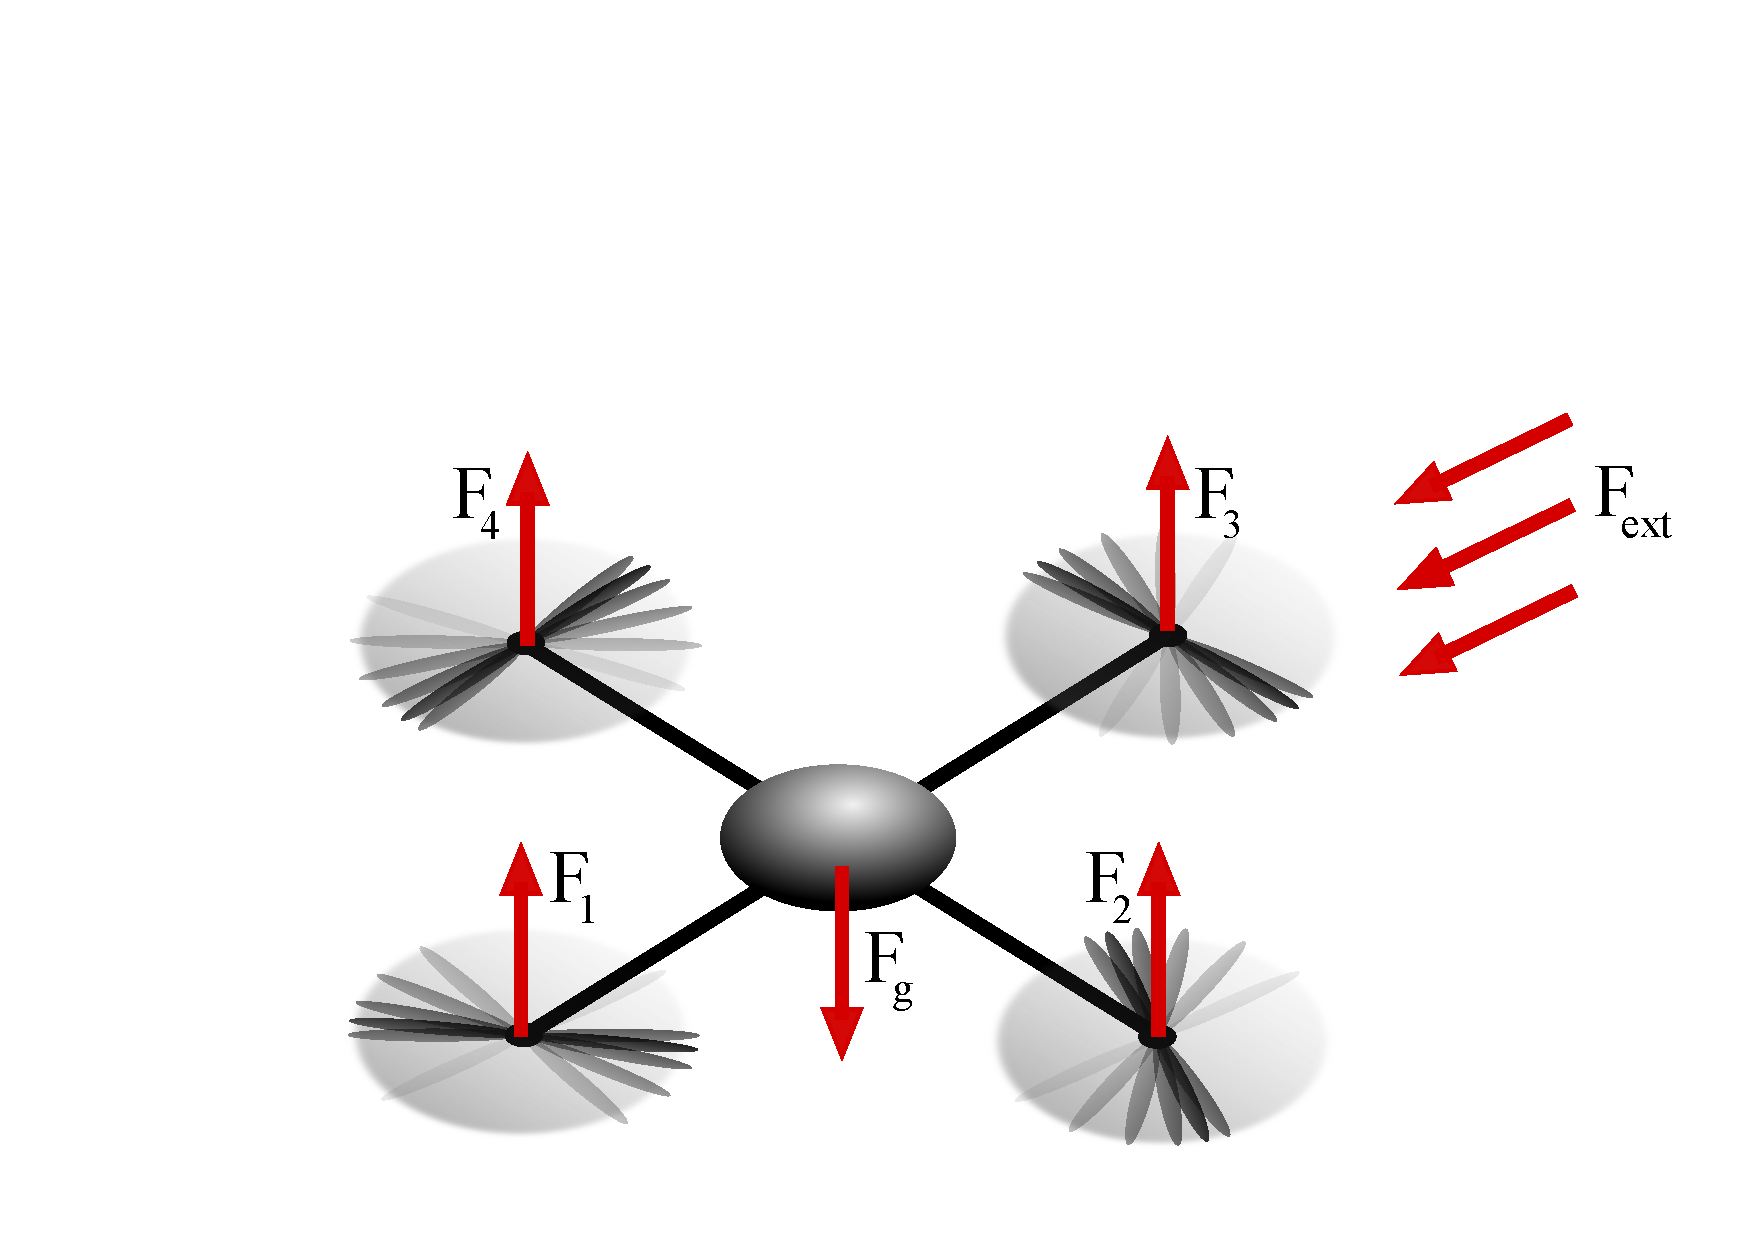
\includegraphics[width=11cm]{images/Copter_Fext_2.pdf}
				\end{textblock}
			\end{column}
			\begin{column}{0.39\textwidth}
				\begin{textblock}{0}(-.7,0.6)
					\[ \mathlarger{F_{res} =F_{ext} + F_{g} + \sum_{i=1}^{4}{F_{i}}} \]
				\end{textblock}
				\end{column}
		\end{columns}
\end{frame}

\begin{frame}
	\frametitle{Torques}
	
			\begin{figure}[p]
					\centering
					\includegraphics<1>[width=11cm]{images/Copter_axis.pdf}
				%
					%\includegraphics<2>[width=11cm]{images/Copter_psi.pdf}
%
					%\includegraphics<3>[width=11cm]{images/Copter_phi.pdf}

					\includegraphics<2>[width=11cm]{images/Copter_theta.pdf}
				\end{figure}
		
\end{frame}

\begin{frame}
		\frametitle{Torques}
			\begin{columns}[T] % align columns
			\begin{column}{.7\textwidth}
				\begin{textblock}{0}(-1,-5.3)
					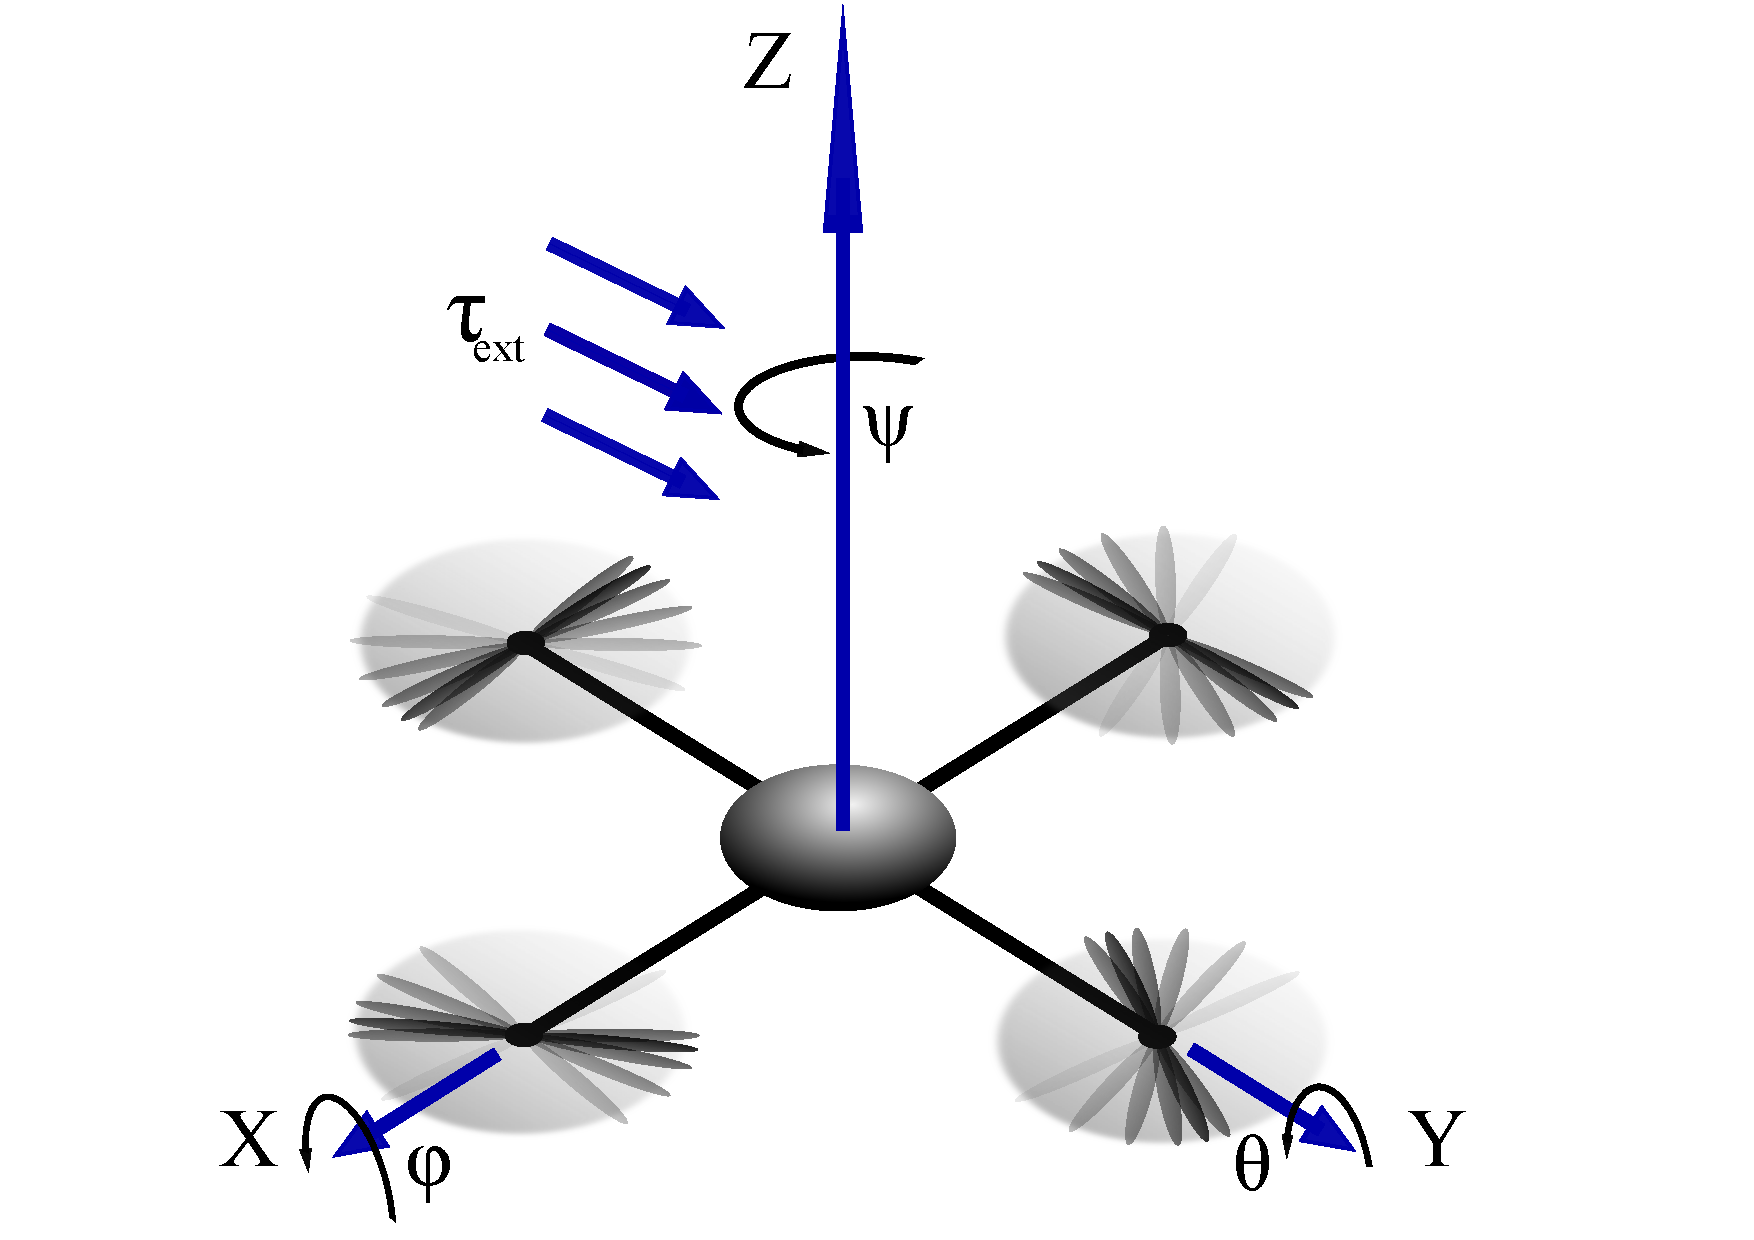
\includegraphics[width=11cm]{images/Copter_Text.pdf}
				\end{textblock}
			\end{column}
			\begin{column}{0.35\textwidth}
				\begin{textblock}{0}(-3,-3.4)
					\[ \mathlarger{\mathlarger{\tau_{res} = \tau_{ext}+\tau_{\psi}+\tau_{\varphi}+\tau_{\theta}}} \]
				\end{textblock}
				\end{column}
		\end{columns}
\end{frame}

\begin{frame}
	\frametitle{Obtain ODE}
	\begin{block}{}
		\centering
		\[\left. \begin{array}{rl} F_{res} \hspace{-1.25ex} &= F_{ext} + F_{g} + \sum_{i=1}^{4}{F_{i}} \\ \tau_{res} \hspace{-1.25ex} &= \tau_{ext} + \tau_{\psi} + \tau_{\varphi} + \tau_{\theta}  \end{array} \right\} \quad \Rightarrow \quad \dot{x}(t)=f(x(t),u(t)) \]
		\vspace{1ex}
	\end{block}
	
	\vspace{2em}
	
	\begin{block}{}
		\begin{center}
		 	\[ \quad \left. \begin{array}{c} \tilde{h}(x,u)=0 \\  \dot{x}(t) = f(x(t),u(t)) \end{array} \right\} \Rightarrow h(x,u) = 0	\]
		\end{center}
		\vspace{1ex}
	\end{block}
	
\end{frame}
